\chapter{Appendix: Other Publications}
\label{chapter:publications}

This part contains the publication outcome of the projects I was collaborating
on during my PhD studies. In total there are 5 publications sorted as the list
by a year in a descending order. Further, each manuscript is represented by
its title page.

\vspace{5mm}

Koča J, Svobodová Vařeková R, Pravda L, Berka K, \underline{Geidl S}, Otyepka M:
\textbf{Structural Bioinformatics Tools for Drug Design}
\textit{Springer International Publishing, Cham} 2016.

\vspace{5mm}

Ionescu CM, Sehnal D, Falginella F L, Pant P, Pravda L, Bouchal T,
Svobodová Vařeková R, \underline{Geidl S}, Koča J: 
\textbf{AtomicChargeCalculator: Interactive Web-based calculation of atomic
charges in large biomolecular complexes and drug like molecules}
\textit{J Cheminform} 2015, \textbf{7}:50.

\vspace{5mm}

Sehnal D, Svobodová Vařeková R, Pravda L, Ionescu CM, \underline{Geidl S},
Horský V, Jaiswal D, Wimmerová M, Koča J: \textbf{ValidatorDB: database of up-to-date
validation results for ligands and non-standard residues from the Protein Data Bank}
\textit{Nucleic Acids Res} 2015, \textbf{43}:D368--D375.

\vspace{5mm}

Svobodová Vařeková R, Jaiswal D, Sehnal D, Ionescu CM, \underline{Geidl S},
Pravda L, Horský V, Wimmerová M, Koča J: \textbf{MotiveValidator: interactive
web-based validation of ligand and residue structure in biomolecular complexes}
\textit{Nucleic Acids Res} 2014, \textbf{42}:W227--W233.


\vspace{5mm}

Ionescu CM, \underline{Geidl S}, Svobodová Vařeková R,Koča J: \textbf{Rapid Calculation
of Accurate Atomic Charges for Proteins via the Electronegativity Equalization Method}
\textit{J Chem Inf Model} 2013, \textbf{53}:10.


\clearpage

%% book
\begin{center}
\section{\centering Structural Bioinformatics Tools for Drug Design}

\subsection*{\centering Extraction of Biologically Relevant Information from Structural Databases}

Jaroslav Koča$^1$, Radka Svobodová Vařeková$^1$, Lukáš Pravda$^1$,
Karel Berka$^2$, \underline{Stanislav Geidl$^1$}, David Sehnal$^1$,
Michal Otyepka$^2$

\vspace{1cm}

$^1$ National Centre for Biomolecular Research, Masaryk University Brno,
Faculty of Science National Centre Biomolecular Research, Brno-Bohunice,
Czech Republic

$^2$ Regional Centre of Advanced Technologies and Materials,
Department of Physical Chemistry, Palacký University Olomouc,
Faculty of Science Olomouc, Czech Republic

\vspace{1cm}

Book in series \textit{SpringerBriefs in Biochemistry and Molecular Biology},
published by \textit{Springer, Cham}, 2016.

\vspace{1cm}

\url{http://doi.org/10.1007/978-3-319-47388-8}

\end{center}

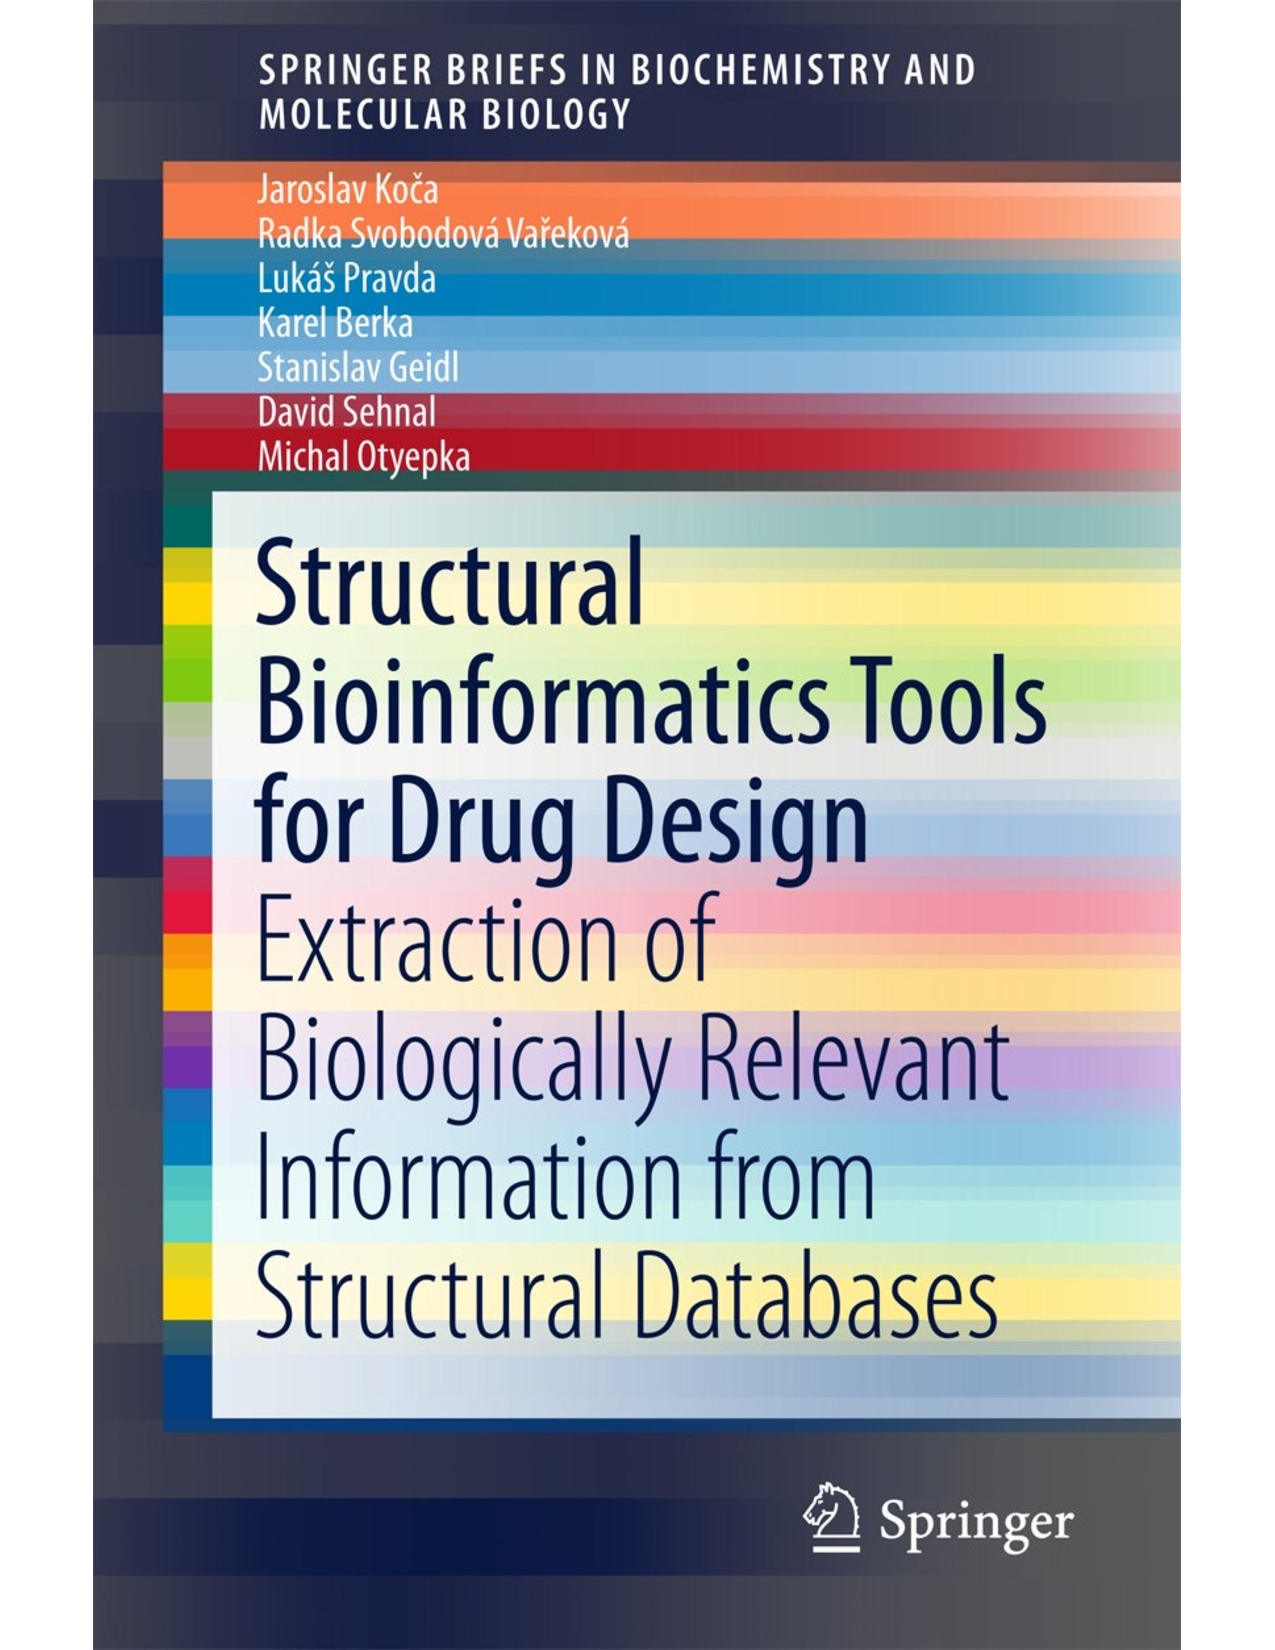
\includepdf[pages=-]{others/book.pdf}

%%% atomic charge calculator
\begin{center}
\section{\centering AtomicChargeCalculator: Interactive Web-based calculation
of atomic charges in large biomolecular complexes and drug like molecules}

Crina-Maria Ionescu$^1$, David Sehnal$^{1, 2, 3}$, Francesco L. Falginella$^1$,
Purbaj Pant$^2$, Lukáš Pravda$^{1, 2}$, Tomáš Bouchal$^{1, 2}$,
Radka Svobodová Vařeková$^{1, 2}$, \underline{Stanislav Geidl}$^{1, 2}$,
Jaroslav Koča$^{1, 2}$

\vspace{1cm}

$^1$ CEITEC -- Central European Institute of Technology,
Masaryk University Brno, Kamenice 5, 625 00 Brno, Czech Republic.

$^2$ National Centre for Biomolecular Research, Faculty of Science,
Masaryk University Brno, Kotlářská 2, 611 37, Brno, Czech Republic.

$^3$ Faculty of Informatics, Masaryk University Brno, Botanická 68a, 602 00 Brno,
Czech Republic.

\vspace{1cm}

\textit{Journal of Cheminformatics} 2015, \textbf{7}:50.

\vspace{1cm}

\url{https://doi.org/10.1186/s13321-015-0099-x}

\end{center}

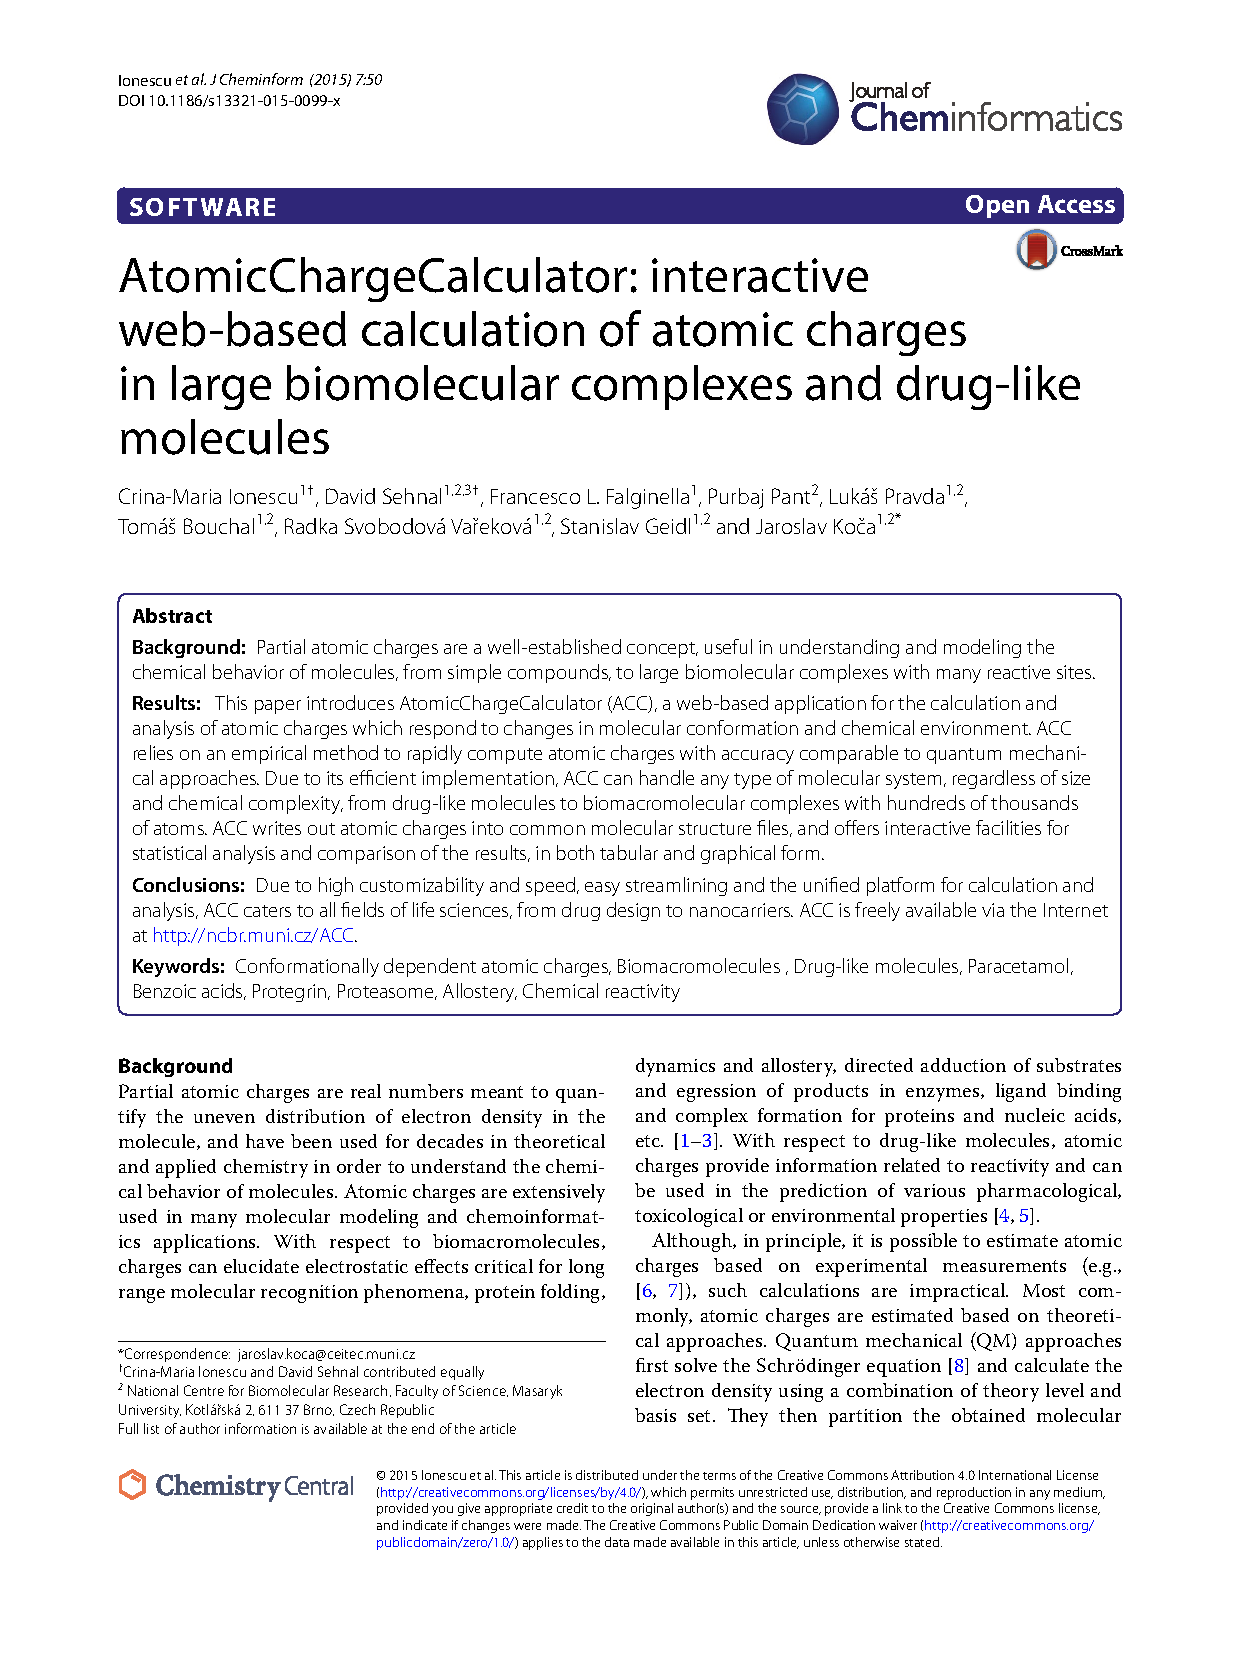
\includepdf[pages=-]{others/charge_calculator.pdf}

%%% validator DB
\begin{center}
\section{\centering ValidatorDB: database of up-to-date
validation results for ligands and non-standard residues from the Protein Data Bank}

David Sehnal$^{1, 2, 3}$,
Radka Svobodová Vařeková$^{1, 2}$,
Lukáš Pravda$^{1, 2}$,
Crina-Maria Ionescu$^1$,
\underline{Stanislav Geidl}$^{1, 2}$,
Vladimír Horský$^3$,
Deepti Jaiswal$^1$,
Michaela Wimmerová$^{1, 2}$,
Jaroslav Koča$^{1, 2}$

\vspace{1cm}

$^1$ CEITEC -- Central European Institute of Technology,
Masaryk University Brno, Kamenice 5, 625 00 Brno, Czech Republic.

$^2$ National Centre for Biomolecular Research, Faculty of Science,
Masaryk University Brno, Kotlářská 2, 611 37, Brno, Czech Republic.

$^3$ Faculty of Informatics, Masaryk University Brno, Botanická 68a, 602 00 Brno,
Czech Republic.

\vspace{1cm}

\textit{Nucleic Acids Research} 2015, \textbf{43}:D368--D375.

\vspace{1cm}

\url{https://doi.org/10.1093/nar/gku1118}

\end{center}

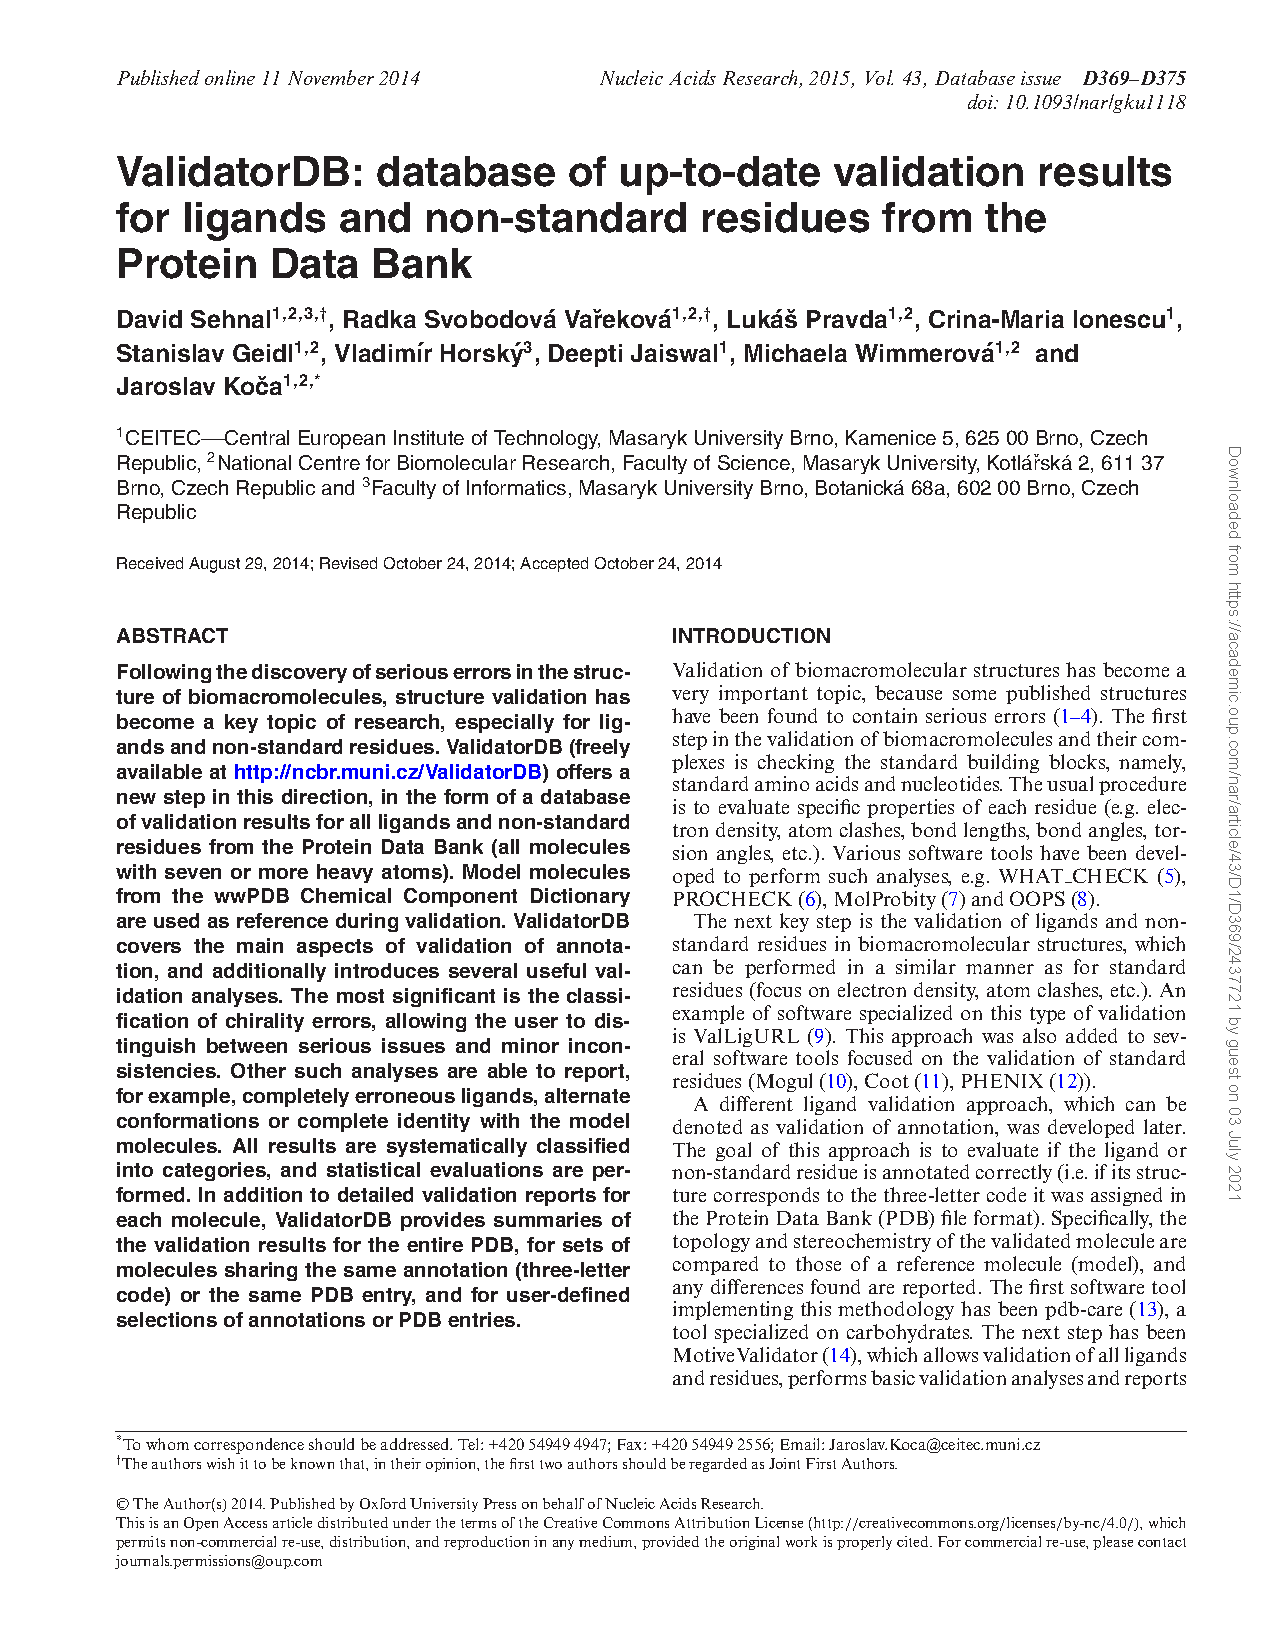
\includepdf[pages=-]{others/validator_db.pdf}

%%% motive validator
\begin{center}
\section{\centering MotiveValidator: interactive
web-based validation of ligand and residue structure in biomolecular complexes}

Radka Svobodová Vařeková$^{1, 2}$,
Deepti Jaiswal$^1$,
David Sehnal$^{1, 2, 3}$,
Crina-Maria Ionescu$^1$,
\underline{Stanislav Geidl}$^{1, 2}$,
Lukáš Pravda$^{1, 2}$,
Vladimír Horský$^3$,
Michaela Wimmerová$^{1, 2}$,
Jaroslav Koča$^{1, 2}$

\vspace{1cm}

$^1$ CEITEC -- Central European Institute of Technology,
Masaryk University Brno, Kamenice 5, 625 00 Brno, Czech Republic.

$^2$ National Centre for Biomolecular Research, Faculty of Science,
Masaryk University Brno, Kotlářská 2, 611 37, Brno, Czech Republic.

$^3$ Faculty of Informatics, Masaryk University Brno, Botanická 68a, 602 00 Brno,
Czech Republic.

\vspace{1cm}

\textit{Nucleic Acids Research} 2015, \textbf{43}:D368--D375.

\vspace{1cm}

\url{https://doi.org/10.1093/nar/gku426}

\end{center}

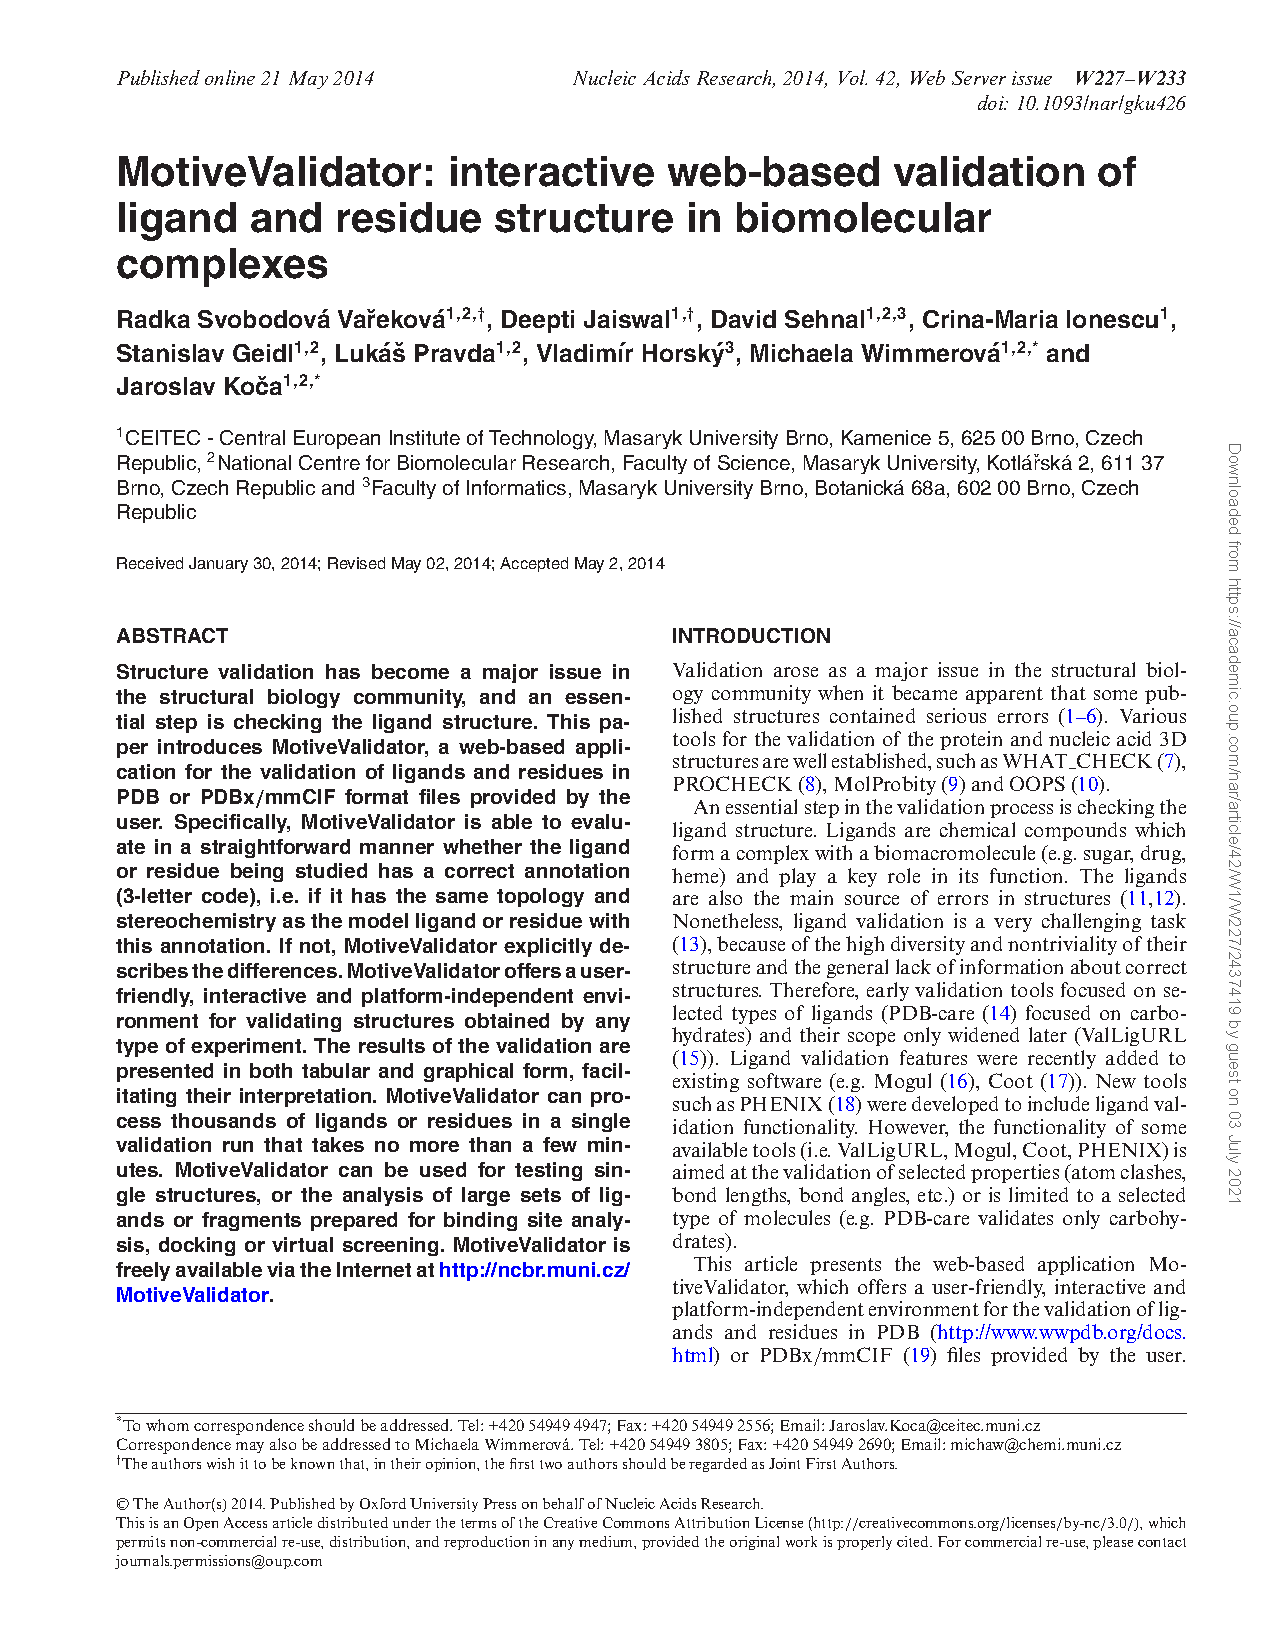
\includepdf[pages=-]{others/motive_validator.pdf}

%%% charges for proteins
\begin{center}
\section{\centering Rapid Calculation of AccurateAtomic Charges
for Proteins via the Electronegativity Equalization Method}

Crina-Maria Ionescu,
\underline{Stanislav Geidl},
Radka Svobodová Vařeková,
Jaroslav Koča

\vspace{1cm}

CEITEC--Central European Institute of Technology, and National
Centre for Biomolecular Research, Faculty of Science, Masaryk
University Brno, Kamenice 5, 625 00 Brno, Czech Republic.

\vspace{1cm}

\textit{Nucleic Acids Research} 2013, \textbf{53}:10.

\vspace{1cm}

\url{https://doi.org/10.1021/ci400448n}

\end{center}

%\includepdf[pages=-]{others/charges_for_proteins.pdf}

